\graphicspath{{content/chapters/7_evaluation/figures/}}
\chapter{Evaluation}
\label{chp:evaluation}

This chapter provides a comprehensive evaluation of the implemented speech enhancement pipeline. The analysis is divided into three major parts: (i) a comparison of dataset handling strategies and their impact on computational efficiency, (ii) an assessment of model performance across dataset variants, and (iii) hyperparameter tuning on the best-performing dataset–model configuration. This layered evaluation approach enables both system-level insight and fine-grained model optimization.

\section{Dataset Performance}
\label{sec:dataset_performance}

This section examines the performance of the three dataset handling strategies—Static Bucketing, Dynamic Bucketing, and Padding-Truncation Output-Truncation (PTO). The goal is to assess how these strategies affect the overall efficiency of the training process, particularly in terms of dataset loading times, runtime overhead during training, and their influence on model performance. Each strategy was tested using the same model architecture, the Contextual Encoder-Decoder (CED), under two conditions:

\begin{itemize}
    \item \textbf{Cold Run (Uncached):} In this scenario, all dataset operations are executed from scratch. Static and Dynamic Bucketing compute bucket assignments (with Dynamic Bucketing also requiring K-Means clustering), while PTO calculates and stores the original waveform lengths. This setup simulates a first-time deployment or training on a fresh system.
    
    \item \textbf{Warm Run (Cached):} This run utilizes cached data generated during the cold run, significantly reducing load and preprocessing time. For Static and Dynamic Bucketing, bucket mappings and K-Means centers are reloaded. For PTO, the previously computed original sequence lengths are retrieved.
\end{itemize}

The configuration used for all runs is shown in Figure~\ref{fig:dataset_config}, with the only varying parameter being the \texttt{PAD\_METHOD}.

\begin{figure}[H]
    \centering
    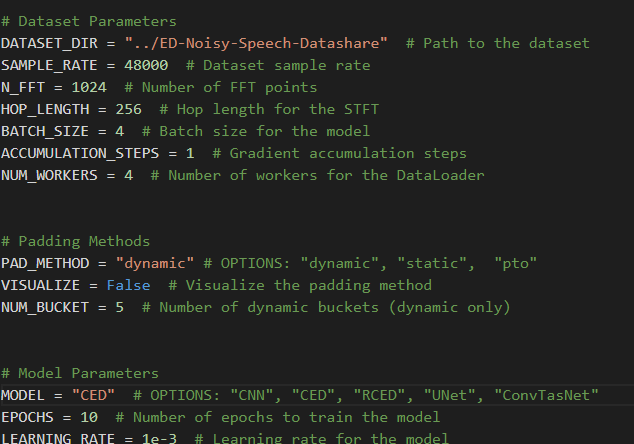
\includegraphics[width=0.8\textwidth]{dataset_config.png}
    \caption{\label{fig:dataset_config} Configuration of the CED model used for dataset performance evaluation.}
\end{figure}

Both uncached and cached runs were executed, and the relevant timing metrics were collected from the output logs, as shown in Table~\ref{tab:dataset_loading_times}.

\vspace{1em}
\begin{table}[H]
\centering
\caption{Training dataset preparation and runtime overheads (in seconds)}
\label{tab:dataset_loading_times}
\begin{tabular}{|l|c|c|c|}
\hline
\textbf{Dataset} & \textbf{Uncached} & \textbf{Cached} & \textbf{Truncation Overhead} \\
\hline
Static Bucketing  & 298.05 s  & 0.81 s   & N/A    \\
Dynamic Bucketing & 602.56 s& 0.58 s  & N/A    \\
PTO               & 311.21 s & 0.58 s  & 58.56 s  \\
\hline
\end{tabular}
\end{table}

The results in Table~\ref{tab:dataset_loading_times} offer a clear overview of the dataset loading times and runtime overheads associated with each method. Static Bucketing proves to be the fastest in terms of initial load time, comprising only dataset loading and bucket assignment. Dynamic Bucketing incurs the highest overhead due to the computational cost of K-Means clustering. PTO, while slightly slower than Static Bucketing, remains efficient given that it must iterate through the dataset to compute the original waveform lengths.

The re-run loading times for all three methods are drastically reduced thanks to the use of cached data. All methods show comparable re-run times, with Static Bucketing being marginally slower.

A key distinction lies in the \textit{epoch truncation overheads}. Only the PTO method incurs this overhead due to its need to truncate outputs during training and evaluation to match the original input lengths. This step is unnecessary for the other two methods. While the added runtime is relatively minor in the context of total training time (typically in the order of hours), this overhead can scale significantly with larger datasets or more training epochs.

To evaluate the impact of dataset handling strategies on model learning, all models were compared using their best training checkpoint. Since the difference between cached and uncached runs was negligible in terms of performance, only the cached results are reported in Table~\ref{tab:dataset_performance}.

\vspace{1em}
\begin{table}[H]
\centering
\caption{Model Training Performance Across Dataset Handling Strategies}
\label{tab:dataset_performance}
\begin{tabular}{|l|c|c|c|}
\hline
\textbf{Dataset} & \textbf{Train Loss} & \textbf{Val Loss} & \textbf{Val SNR} \\
\hline
Static Bucketing  & 0.8367  & 0.8410  & 1.09 dB \\
Dynamic Bucketing & 0.8262  & 0.8298  & 1.10 dB \\  
PTO               & 0.6288  & 0.6633  & 1.10 dB \\
\hline
\end{tabular}
\end{table}

The results in Table~\ref{tab:dataset_performance} indicate that the model achieves comparable performance across all dataset handling methods. The consistent validation SNR values confirm that each method was implemented correctly and that the model learned similar representations regardless of the input formatting.

Interestingly, the PTO method shows a slightly lower training and validation loss. This discrepancy is not reflected in the SNR metric and may be attributed to differences in how output sequences are truncated during training. The closeness of training and validation losses across all configurations suggests that the model generalizes well and is neither underfitting nor overfitting.


\section{OOM Validation}
\label{sec:oom_validation}

While Section~\ref{sec:oom_handling} outlined several techniques to mitigate Out-of-Memory (OOM) errors during training, it is important to demonstrate that these strategies do not compromise model learning. The goal of this section is to validate that memory-saving methods do not lead to information loss or degraded performance.

To assess this, three training configurations were evaluated using the same RCED model architecture and the Dynamic Bucketing dataset strategy:

\begin{enumerate}
    \item \textbf{Clean Training (Baseline):} A standard training loop without any OOM-handling logic, using a batch size of 4. This configuration serves as the control, with no memory management mechanisms.
    
    \item \textbf{OOM Handling (Batch 4, Accum 1):} OOM-handling techniques were enabled while maintaining a batch size of 4. This included fixed-point precision (FP16) and garbage collection (GC), allowing for a more memory-efficient training process.
    
    \item \textbf{OOM + Accumulation (Batch 2, Accum 2):} The batch size was reduced to 2 with gradient accumulation set to 2, simulating an effective batch size of 4. All OOM-handling techniques remained enabled. This configuration is designed to reduce memory usage while preserving gradient stability.
\end{enumerate}

Each configuration was trained for the same number of epochs, using identical learning rates, optimizers, and data augmentation (if any). Table~\ref{tab:oom_training} summarizes the training and validation performance.

\vspace{1em}
\begin{table}[H]
\centering
\caption{Training Performance Across OOM Configurations}
\label{tab:oom_training}
\begin{tabular}{|l|c|c|c|c|}
\hline
\textbf{Train Config} & \textbf{Train Loss} & \textbf{Val Loss} & \textbf{Val SNR} & \textbf{Training Time} \\
\hline
Baseline               & 0.7985 & 0.8048 & 1.12 dB & 4.24 h \\
OOM Handling           & 0.8026 & 0.8077 & 1.11 dB & 2.58 h \\
OOM + Accumulation     & 0.8007 & 0.8077 & 1.11 dB & 3.02 h \\
\hline
\end{tabular}
\end{table}

As shown in Table~\ref{tab:oom_training}, OOM-handling techniques do not significantly affect model performance. Although the training and validation losses are slightly higher than the baseline, the differences are minimal and outweighed by the substantial reduction in training time. This speedup likely results from improved memory efficiency via FP16 computation, garbage collection, and reduced GPU memory overhead.

Each model was also evaluated in the full denoising pipeline. Table~\ref{tab:oom_metrics} presents the performance metrics across key evaluation criteria.

\vspace{1em}
\begin{table}[H]
\centering
\caption{Denoising Metrics Across OOM Configurations}
\label{tab:oom_metrics}
\begin{tabular}{|l|c|c|c|c|c|}
\hline
\textbf{Train Config} & \textbf{↑SNR} & \textbf{↓MSE} & \textbf{↑PESQ} & \textbf{↑STOI} & \textbf{↓LSD} \\
\hline
Baseline               & 0.9751 & 0.002083 & 1.3867 & 0.8205 & 0.7857 \\
OOM Handling           & 0.9648 & 0.002088 & 1.2244 & 0.8037 & 1.0361 \\
OOM + Accumulation     & 0.9714 & 0.002085 & 1.2611 & 0.8044 & 0.9004 \\
\hline
\end{tabular}
\end{table}

Once again, the results in Table~\ref{tab:oom_metrics} confirm that OOM-handling techniques do not degrade model output quality in any significant way. The baseline configuration achieves slightly better metrics, which may be attributed to longer training duration and full-precision computation. However, the differences are negligible, and the gains in training efficiency justify the use of OOM-handling strategies in practice.


\section{Model Performance}
\label{sec:model_performance}

This section presents the most critical part of the evaluation process and the main focus of this project. The compartivive assesment of the classical methods and the five machine learning models performances is shown in this section. Unlike the previous evaluations taken place, which focused on dataset handling strategies and OOM mitigation techniques using fixed models to conduct the implementation justification. However, the main scope of this project is to justify the use of machine learning models for speech enhancement, and to evaluate their performance against classical methods.

The evaluation retains the previously established dynamic bucketing and OOM handling strategies but now focuses on how model design impacts training efficiency and denoising performance. The section begins with an analysis of classical denoising methods to establish a meaningful baseline for comparison.

\subsection{Classical Methods}
\label{sec:classical_methods}

The classical methods evaluated include Spectral Subtraction (SS), Wiener Filtering (WF), and the Minimum Mean Square Error - Log Spectral Amplitude estimator (MMSE-LSA), all implemented in a single-channel setting. SS and WF are well-established in the literature, while MMSE-LSA represents a more recent and perceptually motivated approach. Since these methods do not require training, the classical evaluation bypasses model training and instead focuses solely on denoising performance using the same denosing pipeline and evaluation metrics as the learning-based models.


\vspace{1em}
\begin{table}[H]
\centering
\caption{Classical Denoised Metrics}
\label{tab:classical_metrics}
\begin{tabular}{|l|c|c|c|c|c|c|}
\hline
\textbf{Method} & \textbf{↑SNR} & \textbf{↓MSE} & \textbf{↑PESQ} & \textbf{↑STOI} & \textbf{↓LSD} & \textbf{Denoise Time} \\
\hline
SS          & 1.5406 & 0.002210 & 1.4574 & 0.8538 & 0.7747 & 01.17 m \\
WF          & -3.3796 & 0.006702 & 1.8721 & 0.8968 & 0.9278 & 01.33 m \\
MMSE-LSA    & -2.3929 & 0.005440 & 2.0671 & 0.8974 & 0.8274 & 01.51 m \\
\hline
\end{tabular}
\end{table}


The results in Table~\ref{tab:classical_metrics} highlight key trade-offs between signal fidelity and perceptual quality. SS achieved the best SNR and MSE, suggesting strong numerical suppression of noise. However, it underperformed in perceptual metrics, likely due to spectral distortion and residual artifacts introduced by aggressive subtraction.

In contrast, MMSE-LSA produced the best perceptual outcomes, achieving the highest PESQ and STOI scores, despite a negative SNR. This confirms its ability to preserve intelligibility and speech naturalness, aligning with its design as a perceptually motivated algorithm. WF offered a balanced result, performing reasonably well across all metrics. Notably, all classical methods completed denoising in under two minutes, indicating no significant differences in computational cost. These findings support MMSE-LSA as the most effective classical method overall, particularly for real-world speech enhancement scenarios where perceptual clarity is prioritized.

\subsection{Training Machine Learning Models}
\label{sec:training_ml_models}

With the classical methods evaluated, the focus now shifts to the machine learning models. These models were trained using the same dataset handling strategies and OOM mitigation techniques previously established. Each model followed a consistent training configuration: a batch size of 2, accumulation steps of 4, 25 training epochs, and a learning rate of $1\text{e}{-3}$. The table below summarizes the training performance for each model.

\vspace{1em}
\begin{table}[H]
\centering
\caption{Machine Learning Models Training Performance}
\label{tab:ml_training}
\begin{tabular}{|l|c|c|c|c|}
\hline
\textbf{Model} & \textbf{Train Loss} & \textbf{Val Loss} & \textbf{Val SNR} & \textbf{Training Time} \\
\hline
CNN         & 0.8813 & 0.8883 & 1.06 dB & 3.22 h \\
CED         & 0.8302 & 0.8334 & 1.10 dB & 5.27 h \\
RCED        & 0.8001 & 0.8071 & 1.11 dB & 7.32 h \\
UNet        & 0.7941 & 0.8003 & 1.12 dB & 14.32 h \\
ConvTasNet  & 0.0764 & 0.0760 & 4.76 dB & 13.09 h \\
\hline
\end{tabular}
\end{table}

The results in Table~\ref{tab:ml_training} reveal a steady trend: as model complexity increases, training and validation losses generally decrease, while validation SNR improves. This is particularly evident when moving from CNN to RCED and UNet. Notably, ConvTasNet demonstrates a dramatic jump in validation SNR—from 1.12 dB to 4.76 dB—highlighting its architectural advantage in capturing signal structure. While loss values alone do not fully reflect denoising effectiveness, the ConvTasNet's performance indicates strong generalization and learning during training.

\subsubsection{CNN Training}
\label{sec:cnn_training}

The CNN model was introduced as a simple baseline to validate the project’s training and evaluation pipeline. Despite its minimal architecture, it achieved solid performance and served as a valuable reference point for more complex models.

\begin{figure}[H]
    \centering
    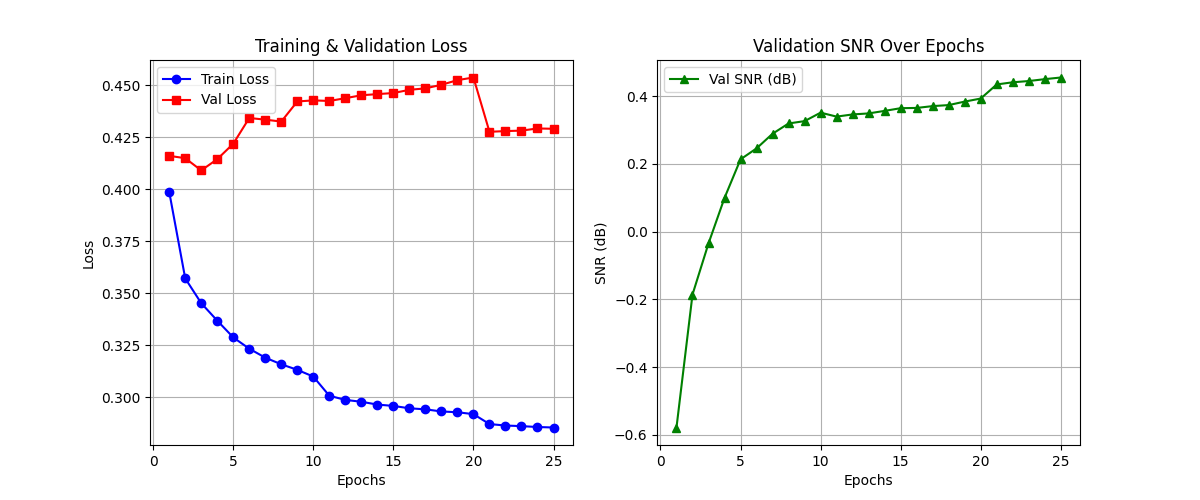
\includegraphics[width=0.8\textwidth]{CNN_plot.png}
    \caption{\label{fig:cnn_training_plot} CNN training plot.}
\end{figure}

The training plot in Figure~\ref{fig:cnn_training_plot} shows a steady upward trend in SNR, indicating consistent learning across epochs. A small gap between training and validation loss is observed, which might suggest mild overfitting. However, the magnitude of this gap (0.007) is negligible, and the model retains good generalization performance, making it a reliable benchmark. The training time of 3.22 hours is reasonable, given the model's simplicity and the dataset size.

\subsubsection{CED Training}
\label{sec:ced_training}


